\section{Structuration}
\sectitle{Structuration des données}

\begin{frame}
    \frametitle{Implémentation du site}

    \begin{itemize}
        \item Développement en \textbf{Symfony} (architecture MVC)
        \item Structuration du code :
            \begin{description}
                \item[Modèle] $\Rightarrow$ Structure des données de l'application
                \item[Vue] $\Rightarrow$ Rendu visuel de l'application
                \item[Contrôleur] $\Rightarrow$ Logique de l'application
            \end{description}
    \end{itemize}
    \begin{figure}
        \centering
        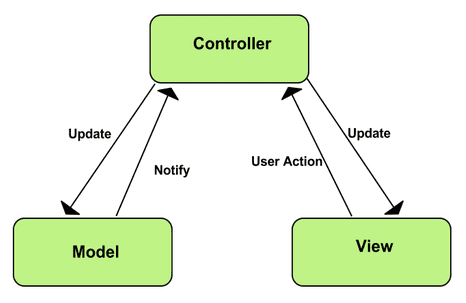
\includegraphics[width=0.5\textwidth]{pictures/mvc-generic.png}
    \end{figure}
\end{frame}

\begin{frame}
    \frametitle{Architecture MVC}

    \centering
    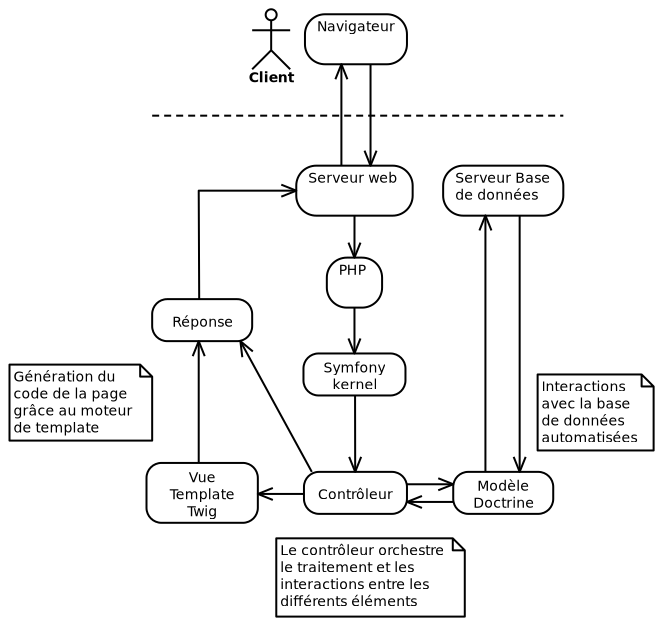
\includegraphics[width=0.7\linewidth]{pictures/mvc.png}
    %\caption{Architecture MVC dans Symfony}
\end{frame}

\begin{frame}
    \frametitle{Redondance des événements}
    \begin{columns}
        \column{0.6\textwidth}
        Le constat :
        \begin{itemize}
            \item Événements redondants
            \item Informations dupliquées
        \end{itemize}
        \pause
        \vspace{2em}
        Notre choix :
        \begin{itemize}
            \item Événements fixes et intemporels
            \item Nouvelle éditions chaque année
        \end{itemize}

        \column{0.4\textwidth}
        \begin{figure}
            \centering
            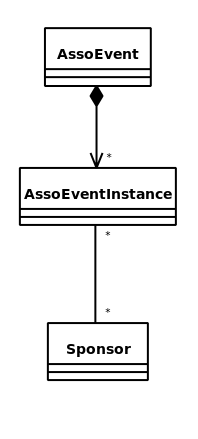
\includegraphics[width=0.6\columnwidth]{pictures/assoevent-struct.png}
        \end{figure}
    \end{columns}
\end{frame}

\begin{frame}
    \frametitle{Redondance des formulaires}
    Le constat :
    \begin{itemize}
        \item Besoins spécifiques pour chaque événement
        \item Formulaires souvent similaires
    \end{itemize}
    \pause
    \vspace{2em}
    Notre choix :
    \begin{itemize}
        \item Formulaires personnalisables \& réutilisables
        \item Construction récursive
    \end{itemize}
\end{frame}

\begin{frame}
    \frametitle{Gestion de la récurtion}
    Généralisation d'un formulaire $\Longrightarrow$ \textit{\textbf{FormWidget}} \vspace{3em}
    \pause
    \begin{columns}
        \column[b]{0.5\textwidth}
        3 types de \textit{FormWidget} :
        \begin{itemize}
            \item<3-> \alert<3>{Natif}
            \item<4-> \alert<4>{Composite}
            \item<5-> \alert<5>{Liste}
        \end{itemize}

        \column{0.5\textwidth}
        \begin{figure}
            \centering
            \includegraphics<3>[width=\columnwidth]{pictures/formwidget-natif.png}
            \includegraphics<4>[width=\columnwidth]{pictures/formwidget-composite.png}
            \includegraphics<5>[width=\columnwidth]{pictures/formwidget-liste.png}
        \end{figure}
    \end{columns}
\end{frame}

\begin{frame}
    \frametitle{Example de construction de formulaire}
    \begin{figure}
        \centering
        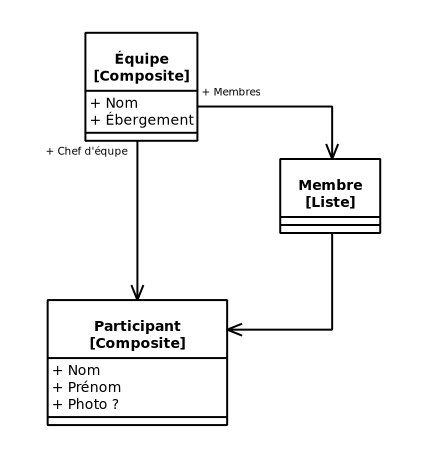
\includegraphics[width=0.65\textwidth]{pictures/formwidget-struct-example.png}
    \end{figure}
\end{frame}

\begin{frame}
    \frametitle{En résumé}
    Structure finale de la base de données :
    \begin{figure}
        \centering
        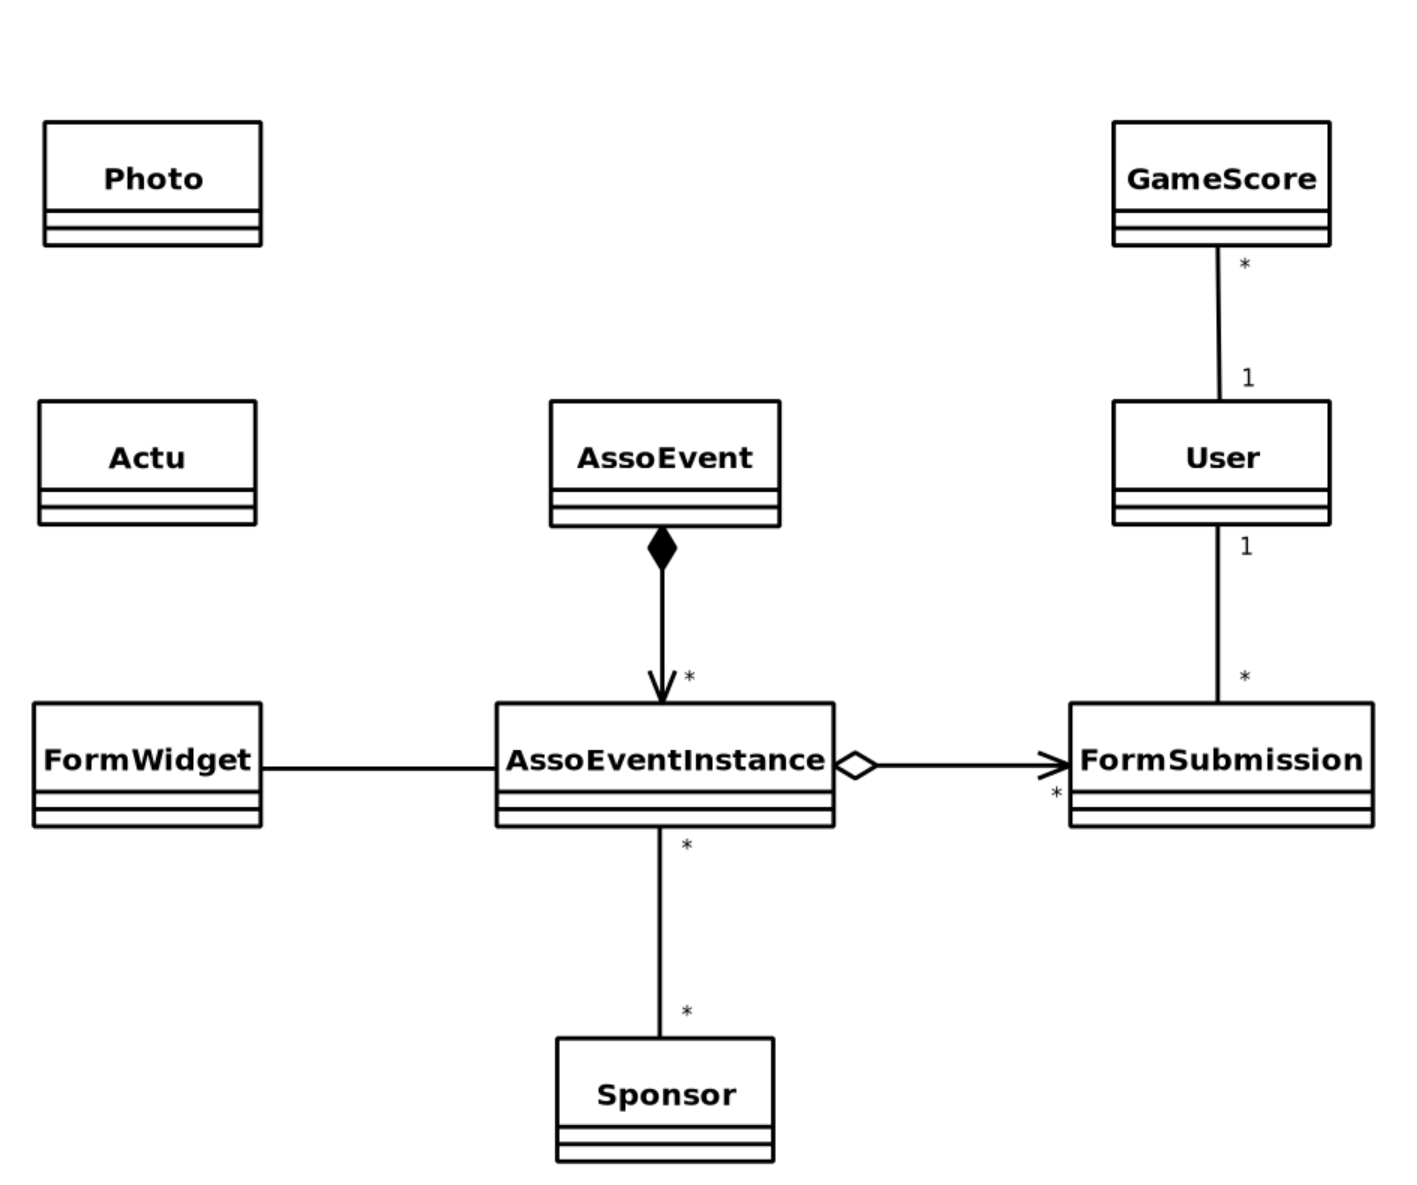
\includegraphics[width=0.8\textwidth]{pictures/database.png}
    \end{figure}
\end{frame}
